\RequirePackage{fix-cm}
\documentclass{bmstu-sob}

% ------------------------------------------------------------
% Подключение стандартных пакетов
% ------------------------------------------------------------
\usepackage{graphicx}
\usepackage{xcolor}

% Настройка стилей для листингов кода
\lstset{
	basicstyle=\small\ttfamily,
	breaklines=true,
	frame=single,
	tabsize=4,
	showstringspaces=false,
	keywordstyle=\color{blue},
	commentstyle=\color{gray},
	stringstyle=\color{teal}
}

% ------------------------------------------------------------
% Нумерация разделов без привязки к главам
% ------------------------------------------------------------
\renewcommand{\thesection}{\arabic{section}}
\renewcommand{\thesubsection}{\arabic{section}.\arabic{subsection}}

% ------------------------------------------------------------
% Документ
% ------------------------------------------------------------
\begin{document}
	
	% ------------------------------------------------------------
	% Титульный лист (используем \input вместо \include)
	% ------------------------------------------------------------
	\makereporttitle
{Платформенные решения для интеллектуального анализа больших данных}
{Компьютерные системы и сети}
{домашней работе №~1}
{Математические методы анализа данных и принятия решений}
{Бинарная кластеризация классическим алгоритмом k-means}
{8}
{Соболев ~Н.~А./ИУ6-13М}
{Тверская~Е.~С.}

	
	% ============================================================
	% 1. ЦЕЛЬ РАБОТЫ
	% ============================================================
	
	\section{Цель работы}
	
	классическим алгоритмом k-means провести процесс бинарной кластеризации предложенных множеств. Проанализировать полученный результат, сделать выводы.
	
	% ============================================================
	% 2. ПОСТАНОВКА ЗАДАЧИ И ИСХОДНЫЕ ДАННЫЕ
	% ============================================================
	
	\section{Постановка задачи и исходные данные}
	
	В соответствии с Вариантом №~8 исходная выборка представляет собой двухмерный массив объектов объема $N = 100$ точек, состоящий из двух кластеров ($K = 2$) со следующими генеральными параметрами:
	\begin{itemize}
		\item Истинные центры кластеров: $\mu_1 = (0.20, 3.00)$, $\mu_2 = (1.00, 3.00)$;
		\item Среднеквадратические отклонения первого кластера: $\sigma_1 = (0.07, 0.50)$;
		\item Среднеквадратические отклонения второго кластера: $\sigma_2 = (0.06, 0.50)$;
		\item Начальные опорные объекты: $z_1^{(0)} = X[1]$, $z_2^{(0)} = X[3]$.
	\end{itemize}
	
	Кластеры анизотропны и сильно вытянуты вдоль вертикальной оси $x_2$ ($\sigma_y \gg \sigma_x$), при этом расстояние между центрами по горизонтальной оси составляет $\Delta x_1 = 0.8$.
	
	% ============================================================
	% 3. ТЕОРЕТИЧЕСКИЙ БАЗИС АЛГОРИТМА K-MEANS И КРИТЕРИИ КАЧЕСТВА
	% ============================================================
	
	\section{Теоретический базис алгоритма k-means}
	
	Алгоритм k-means осуществляет разбиение множества объектов на $K$ кластеров $\{S_1, \dots, S_K\}$ путем минимизации суммарного квадратичного отклонения:
	\begin{equation}
		J = \sum_{j=1}^{K} \sum_{x \in S_j} ||x - m_j||^2 \rightarrow \min
	\end{equation}
	где $m_j$ --- центроид (вектор выборочного среднего) кластера $S_j$.
	
	В классической реализации используется стандартное евклидово расстояние:
	\begin{equation}
		d_E(x, z) = \sqrt{\sum_{k=1}^{n} (x^{(k)} - z^{(k)})^2}
	\end{equation}
	
	Применение евклидова расстояния теоретически обосновано только при условии сферичности порождающих распределений, когда ковариационная матрица имеет вид $\Sigma = \sigma^2 I$.
	
	Для количественной оценки качества разбиения используется внутрикластерная сумма квадратов (WCSS --- Within-Cluster Sum of Squares):
	\begin{equation}
		\text{WCSS} = \sum_{j=1}^{K} \sum_{x \in S_j} d(x, z_j)^2
	\end{equation}
	
	% ============================================================
	% 4. ЭКСПЕРИМЕНТ 1. БАЗОВАЯ РЕАЛИЗАЦИЯ И АНАЛИЗ СБОЯ
	% ============================================================
	
	\section{Эксперимент 1. Базовая реализация алгоритма k-means}
	
	Программная реализация классического алгоритма k-means на языке Python представлена ниже:
	
	\begin{lstlisting}[language=Python]
		import numpy as np
		from sklearn.datasets import make_blobs
		
		# Генерация данных (Вариант 8)
		np.random.seed(0)
		X, _ = make_blobs(
		n_samples=100,
		centers=[(0.2, 3), (1.0, 3)],
		cluster_std=[(0.07, 0.5), (0.06, 0.5)],
		random_state=3
		)
		
		# Инициализация центроидов
		z1 = np.array([X[1], X[3]]).copy()
		
		for iteration in range(100):
		dist0 = np.linalg.norm(X - z1[0], axis=1)
		dist1 = np.linalg.norm(X - z1[1], axis=1)
		labels1 = np.where(dist0 < dist1, 0, 1)
		
		new_z = np.array([X[labels1 == 0].mean(axis=0),
		X[labels1 == 1].mean(axis=0)])
		
		if np.allclose(z1, new_z, atol=1e-5):
		break
		z1 = new_z.copy()
		
		# Расчет ошибки WCSS для классического k-means
		wcss_classic = np.sum([np.sum((X[labels1 == i] - z1[i])**2) for i in range(2)])
	\end{lstlisting}
	
	Результат работы классического алгоритма представлен на рисунке~\ref{fig:kmeans_classic}.
	
	\begin{figure}[htbp]
		\centering
		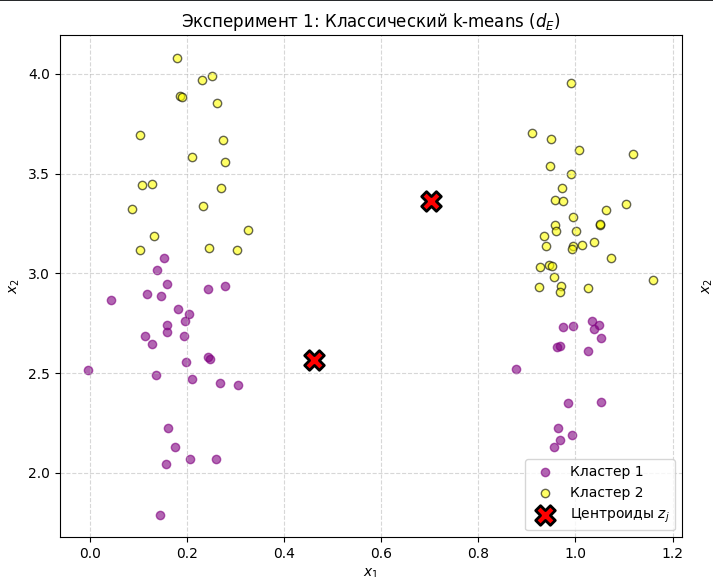
\includegraphics[width=0.85\textwidth]{img/kmeans_classic.png}
		\caption{Результат работы классического алгоритма k-means ($d_E$)}
		\label{fig:kmeans_classic}
	\end{figure}
	
	Вычисленные центры сошлись к значениям $z_1 \approx (0.43, 2.58)$ и $z_2 \approx (0.72, 3.36)$. Разделяющая граница прошла по диагонали, разрезав оба естественных кластера.
	
	% ============================================================
	% 5. ЭКСПЕРИМЕНТ 2. МОДИФИКАЦИЯ МЕТРИКИ
	% ============================================================
	
	\section{Эксперимент 2. Модификация метрики расстояния}
	
	Для устранения влияния высокого разброса по оси ординат $x_2$ использовано взвешенное евклидово расстояние:
	\begin{equation}
		d_{wE}(x, z) = \sqrt{\sum_{k=1}^{n} w_k (x^{(k)} - z^{(k)})^2}
	\end{equation}
	где вектор весовых коэффициентов принят равным $w = (1.0, 0.1)$.
	
	Программный код взвешенного алгоритма:
	
	\begin{lstlisting}[language=Python]
		w = np.array([1.0, 0.1])
		z2 = np.array([X[1], X[3]]).copy()
		
		for iteration in range(100):
		dist0_w = np.sqrt(np.sum(w * ((X - z2[0])**2), axis=1))
		dist1_w = np.sqrt(np.sum(w * ((X - z2[1])**2), axis=1))
		labels2 = np.where(dist0_w < dist1_w, 0, 1)
		
		new_z = np.array([X[labels2 == 0].mean(axis=0),
		X[labels2 == 1].mean(axis=0)])
		
		if np.allclose(z2, new_z, atol=1e-5):
		break
		z2 = new_z.copy()
		
		# Расчет ошибки WCSS для взвешенного k-means
		wcss_weighted = np.sum([np.sum(w * (X[labels2 == i] - z2[i])**2) for i in range(2)])
	\end{lstlisting}
	
	Результат кластеризации с использованием метрики $d_{wE}$ приведен на рисунке~\ref{fig:kmeans_weighted}.
	
	\begin{figure}[htbp]
		\centering
		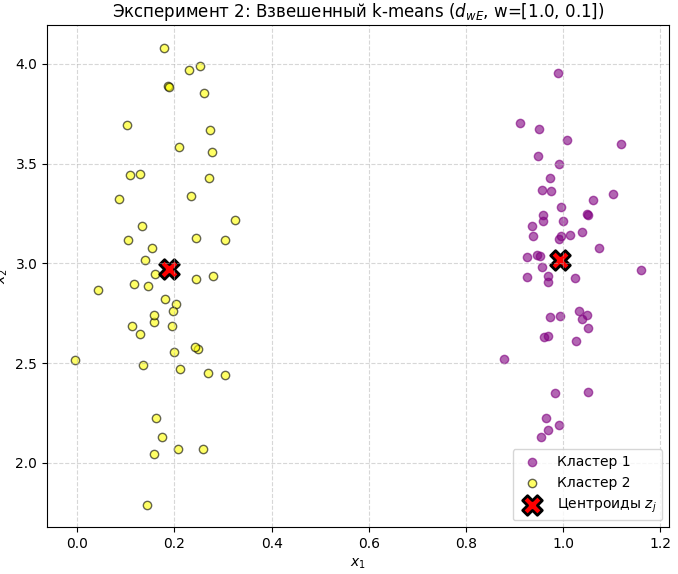
\includegraphics[width=0.85\textwidth]{img/kmeans_weighted.png}
		\caption{Результат работы алгоритма k-means с метрикой $d_{wE}$}
		\label{fig:kmeans_weighted}
	\end{figure}
	
	Введение весовых коэффициентов позволило провести разделяющую границу строго вертикально. Найденные центроиды $z_1 \approx (0.19, 2.98)$ и $z_2 \approx (1.00, 3.01)$ совпали с истинными центрами генерации.
	
	% ============================================================
	% 6. СРАВНИТЕЛЬНЫЙ АНАЛИЗ И МЕТРИКА ОШИБКИ
	% ============================================================
	
	\section{Сравнительный анализ и оценка качества}
	
	Для количественного обоснования эффективности предложенного подхода произведено сравнение суммарных внутрикластерных ошибок WCSS. На рисунке~\ref{fig:wcss_comparison} показано сравнение величины WCSS для обоих методов.
	
	\begin{figure}[htbp]
		\centering
		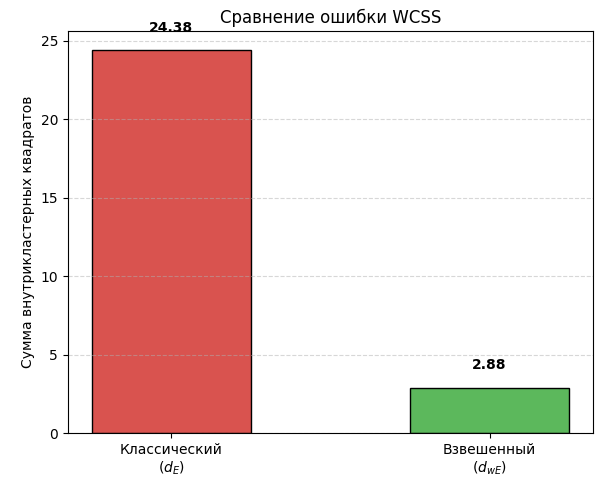
\includegraphics[width=0.65\textwidth]{img/wcss_comparison.png}
		\caption{Сравнение ошибки WCSS для классического и взвешенного k-means}
		\label{fig:wcss_comparison}
	\end{figure}
	
	Сводные результаты проведенных экспериментов приведены в таблице~\ref{tab:comparison}.
	
	\begin{table}[htbp]
		\centering
		\caption{Сравнение точности и метрик алгоритмов}
		\label{tab:comparison}
		\begin{tabular}{|l|c|c|c|}
			\hline
			\textbf{Параметр} & \textbf{Истинный} & \textbf{Классический $d_E$} & \textbf{Взвешенный $d_{wE}$} \\ \hline
			Центроид $z_1$ & $(0.20, 3.00)$ & $(0.43, 2.58)$ & $(0.19, 2.98)$ \\ \hline
			Центроид $z_2$ & $(1.00, 3.00)$ & $(0.72, 3.36)$ & $(1.00, 3.01)$ \\ \hline
			Граница раздела & Вертикальная & Диагональная & Вертикальная \\ \hline
			Ошибка WCSS & --- & $24.38$ & $2.88$ \\ \hline
		\end{tabular}
	\end{table}
	
	% ============================================================
	% 7. ВЫВОД
	% ============================================================
	
	\section{Вывод}
	
	В ходе выполнения работы были сделаны следующие заключения:
	\begin{enumerate}
		\item \textbf{Причина неэффективности классического k-means:} Использование евклидовой метрики $d_E$ предполагает сферическую симметрию кластеров. На анизотропных данных ($\sigma_y / \sigma_x \approx 8.33$) алгоритм разрезает вертикальные кластеры по диагонали, что приводит к некорректному определению центроидов и высокой внутрикластерной ошибке ($\text{WCSS} = 24.38$).
		
		\item \textbf{Эффективность весовой коррекции:} Введение весов $w = (1.0, 0.1)$ компенсирует разницу масштабов по осям, снижая внутрикластерную ошибку почти в 8.5 раз ($\text{WCSS} = 2.88$) и обеспечивая полное восстановление истинного положения центроидов $z_1 \approx (0.19, 2.98)$ и $z_2 \approx (1.00, 3.01)$.
	\end{enumerate}
	
\end{document}